%%%%%%%%%%%%%%%%%%%% book.tex %%%%%%%%%%%%%%%%%%%%%%%%%%%%%
%  root file for the chapters
%%%%%%%%%%%%%%%%%%%%%%%%%%%%%%%%%%%%%%%%%%%%%%%%%%%%%%%%%%%
\documentclass[envcountsame,envcountchap]{svmono}

% choose options for [] as required from the list
% in the Reference Guide, Sect. 2.2

\usepackage{makeidx}         % allows index generation
\usepackage{graphicx}        % standard LaTeX graphics tool
                             % when including figure files
\usepackage{multicol}        % used for the two-column index
\usepackage[bottom]{footmisc}% places footnotes at page bottom
% etc.
% see the list of further useful packages
% in the Reference Guide, Sects. 2.3, 3.1-3.3
% Pakiety dołączane do artykułu TEWI - lista do przejrzenia
\usepackage{polski}
\usepackage{amsmath}
\usepackage{amssymb}
\usepackage{amsfonts}
\usepackage{listings}
\usepackage[svgnames]{xcolor}


\usepackage[utf8]{inputenc}
\usepackage[T1]{fontenc}
\usepackage{graphicx}
\usepackage{amsthm}
\usepackage{txfonts}
\usepackage{epstopdf}
\usepackage{placeins}
\usepackage[english]{babel}
\usepackage[utf8]{inputenc}
\usepackage{array}
\usepackage{subcaption}
\captionsetup{compatibility=false}%http://tex.stackexchange.com/questions/31906/subcaption-package-compatibility-issue

 \lstset{literate={ą}{{\k{a}}}1 {ć}{{\'c}}1 {ę}{{\k{e}}}1 {ł}{{\l{}}}1 {ń}{{\'n}}1 {ó}{{\'o}}1 {ś}{{\'s}}1 {ż}{{\.z}}1 {ź}{{\'z}}1 {Ą}{{\k{A}}}1 {Ć}{{\'C}}1 {Ę}{{\k{E}}}1 {Ł}{{\L{}}}1 {Ń}{{\'N}}1 {Ó}{{\'O}}1 {Ś}{{\'S}}1 {Ż}{{\.Z}}1 {Ź}{{\'Z}}1 }
 \lstset{breaklines=true}
\lstset{language=Matlab,
  keywords={break,case,catch,continue,else,elseif,end,for,function,
     global,if,otherwise,persistent,return,switch,try,while},
  basicstyle=\ttfamily,
  keywordstyle=\color{blue},
  commentstyle=\color{DarkGreen},
  stringstyle=\color{dkgreen},
  numbers=left,
  numberstyle=\tiny\color{gray},
  stepnumber=1,
  numbersep=10pt,
  backgroundcolor=\color{white},
  tabsize=4,
  showspaces=false,
  showstringspaces=false}

% ^^^^^^^Pakiety dołączane do artykułu TEWI - powyższa lista do przejrzenia^^^^^^^


\makeindex             % used for the subject index
                       % please use the style svind.ist with
                       % your makeindex program

%%%%%%%%%%%%%%%%%%%%%%%%%%%%%%%%%%%%%%%%%%%%%%%%%%%%%%%%%%%%%%%%%%%%%

\begin{document}

\author{Antoni Wiliński, Aneta Bera, Katarzyna Buda, Piotr Błaszyński, Łukasz Brzosko, Kamil Knyszyński, Wojciech Nowicki, Tomasz Nyczaj, Artur Pietrzyk, Anton Smoliński, Michał Zabłocki}
\title{Badania algorytmicznych strategii inwestycyjnych???\\
{\small Praca wykonana w ramach projektu TEWI finansowanego z Programu Operacyjnego Innowacyjna Gospodarka w latach 2012-2013}}
\subtitle{-- Podtytuł --}
\maketitle

\frontmatter%%%%%%%%%%%%%%%%%%%%%%%%%%%%%%%%%%%%%%%%%%%%%%%%%%%%%%


%%%%%%%%%%%%%%%%%%%%%%% dedic.tex %%%%%%%%%%%%%%%%%%%%%%%%%%%%%%%%%
% dedication
%%%%%%%%%%%%%%%%%%%%%%%%%%%%%%%%%%%%%%%%%%%%%%%%%%%%%%%%%%%%%%%%%%%

\thispagestyle{empty}
\vspace*{3.5cm}
\begin{flushright}

{\large Miejsce na dedykacje}

\end{flushright}




\include{pref}

\tableofcontents


\mainmatter%%%%%%%%%%%%%%%%%%%%%%%%%%%%%%%%%%%%%%%%%%%%%%%%%%%%%%%
\include{part}
%%%%%%%%%%%%%%%%%%%%% chapter.tex %%%%%%%%%%%%%%%%%%%%%%%%%%%%%%%%%


\chapter{Technical analysis indicators}
\label{Indicators} % Always give a unique label
% use \chaptermark{}
% to alter or adjust the chapter heading in the running head

W poniższym rozdziale zaprezentowane zostaną wskaźniki analizy technicznej oraz ich zastosowanie do handlu na wybranych parach walutowych, indeksach giełdowych i kontraktach terminowych.

\section{ROC --- Rate Of Change indicator}
\label{sec:1ROC}
Rate Of Change is an indicator which measures the percentage change between the latest price and closing price of $k$ periods before. The method of calculating the value of the ROC, for a given point in time, represent formulas \ref{wzorroc_1} and \ref{wzorroc_2}.
\begin{equation}
ROC(\text{now}) = \frac{\text{Current close price} - \text{Close price} k \text{ periods before}}{\text{Close price } k \text{ periods before}}\\
\label{wzorroc_1}
\end{equation}
\begin{equation}
ROC(i) = \frac{C(i,4) - C(i-k,4)}{C(i-k,4)}
\label{wzorroc_2}
\end{equation}

\noindent The basic properties of the ROC curve are:
\begin{itemize}
\item it shows how the observed market price during the period changed,
\item when the oscillator value is below zero, then the current price is higher than one from $k$-candles ago; analogically, when the oscillator is above zero, it means that the current price is lower than the price from $k$-candles ago,
\item increasing indicator line shows that the differences between the current prices and ones from $k$-time ago are increasing, decreasing says, that this differences decrease,
\item if the stock prices rise it can be expected that the oscillator line will behave in the same way; if the prices decrease the oscillator line should decrease.
\end{itemize}
The most important property of the described indicator, used while implementing  the strategy, is that it indicates the moments in which transactions should be made. When the value of the indicator crosses the zero level from below, it is assumed that this is a good time to buy, if it crosses the zero level from above, this is the good time to sale. This is shown in Figure \ref{kupsprzroc}.\\
\begin{figure}[h!]
\centering
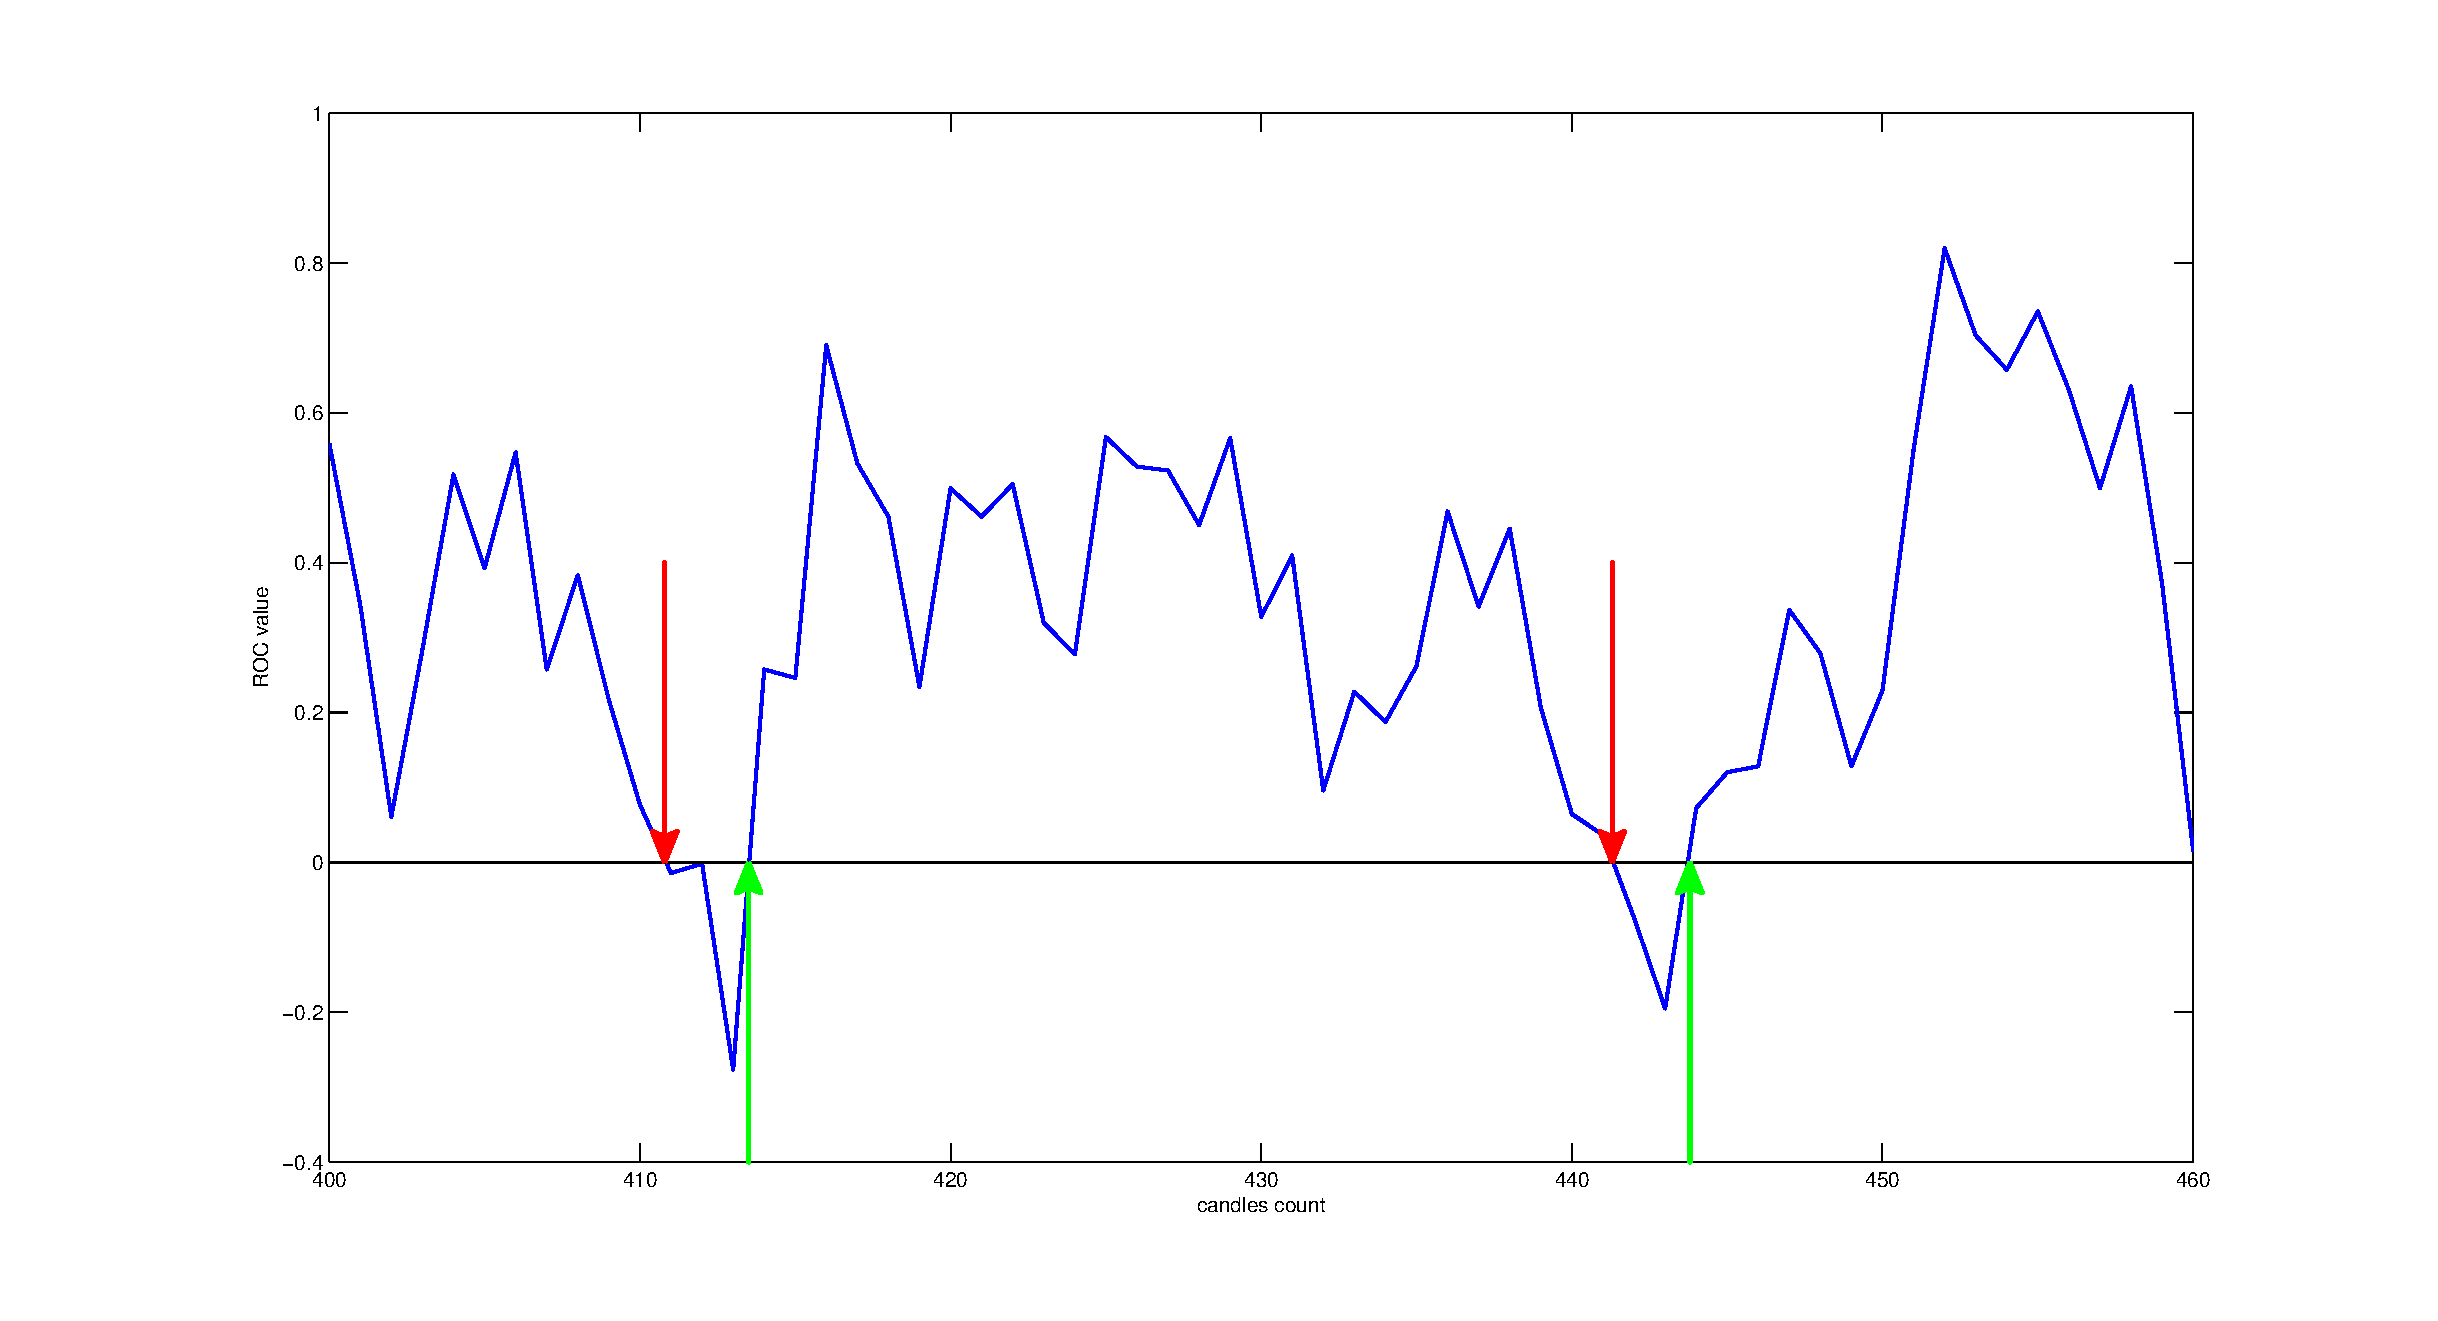
\includegraphics[width = \textwidth]{BuySell.eps}
\caption{Part of the sample ROC curve with buying signals --- green arrows --- and selling signals --- red arrows}
\label{kupsprzroc}
\end{figure}
\FloatBarrier

\noindent The following listing shows the strategy implemented in MATLAB.
\begin{scriptsize}
\begin{lstlisting}
pocz = k+2;	
kon = size(C,1)-1;
iL = 0; % exceeding 0 to top - buy(L)
iS = 0; % exceeding 0 to bottom - sell(S)
sumR = zeros(1,size(C,1));
R = zeros(1,size(C,1));
ROC_vec = zeros(1,kon-k+1);
ROC_vec(pocz-1) = ((C(pocz-1,4) - C(pocz-1-k,4))/C(pocz-1-k,4))*100;

recordReturn = 0;  % record profit
recordDrawdown = 0;  % record drawdown
LastPos = 0;    % variable used to store the value of the opening of the last position

for i=pocz:kon
   ROC_vec(i) = ((C(i,4) - C(i-k,4))/C(i-k,4))*100;  % calculating the ROC curve
   if ROC_vec(i)*ROC_vec(i-1)<=0   % the intersection of the ROC curve with zero
       if ROC_vec(i-1)<ROC_vec(i)  % a condition of purchase
           if iL+iS>0
               R(i) = -C(i+1,4)+LastPos-spread;   % closing S
           end
           LastPos = C(i+1,1);   % open L
           iL = iL + 1;
       elseif ROC_vec(i-1)>ROC_vec(i)  % a condition of sale
           if iL+iS>0
               R(i) = C(i+1,4)-LastPos-spread;  % closing L
           end
           LastPos = C(i+1,1);   % open S
           iS = iS + 1;
       end
   end
   sumR(i) = sum(R(pocz:i));
    if sumR(i)>recordReturn
       recordReturn=sumR(i);
   end
  
   if sumR(i)-recordReturn<recordDrawdown
       recordDrawdown=sumR(i)-recordReturn; 
   end

end

Calmar=-sumR(kon)/recordDrawdown;
profit = sumR(kon);

end
\end{lstlisting}
\end{scriptsize}


Based on collected information on the $ROC$ ratio a simple investment strategy, based on the rule: if the $ROC$ line intersects the zero level from below, it opens a long position ($L$) and closed a short position ($S$) which has been previously opened, was created. When $ROC$ line intersects zero level from above it will open a short position and close a long one. Tests were carried out on $EURJPY$ currency pair (time series shown in Figure \ref{rysunek2roc}).\\

\begin{figure}[h!]
\centering
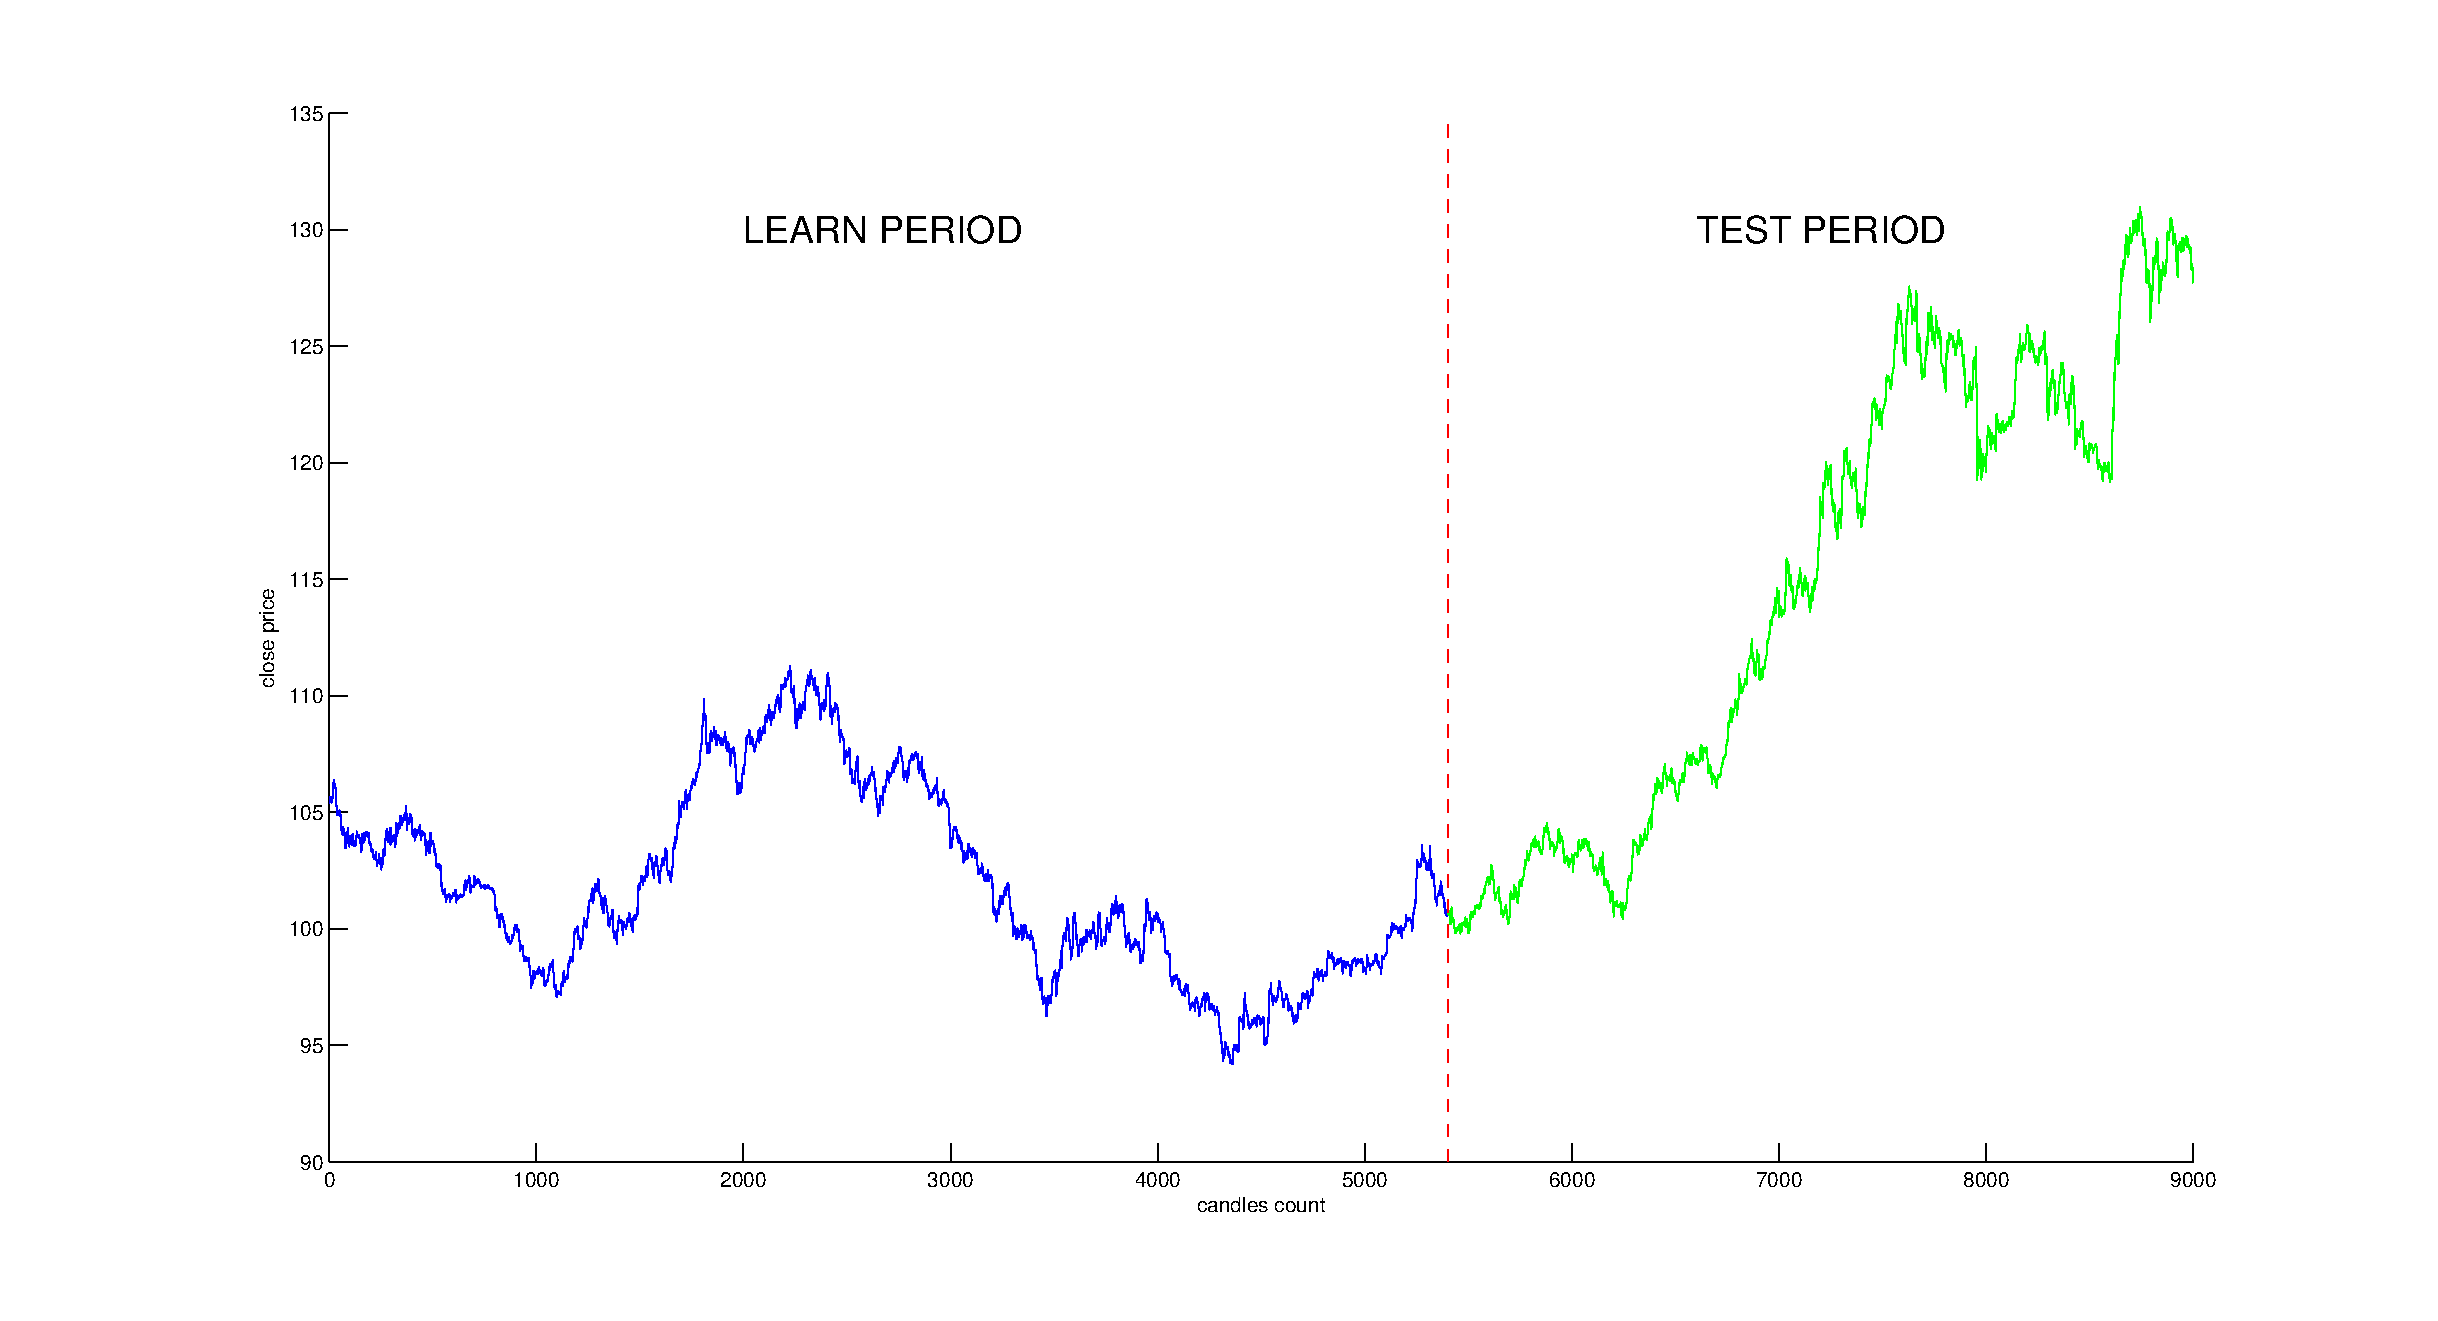
\includegraphics[width = \textwidth]{podzialDanych.eps}
\caption{Studied time series with the division into the learn and test part}
\label{rysunek2roc}
\end{figure}
\FloatBarrier
The entire data set (candles) is divided into two parts: the learn ($60 \%$ of the total) and test ($40\%$ of the total). During studies an optimal value for $k$ on a period of learning was searched, then verified obtained results for the test period. Selecting the optimal value of the parameter $ k $ was determined in two ways:
\begin{itemize}
\item the resulting final profit,
\item Calmar ratio.
\end{itemize}
\newpage
\noindent \textbf{I The results of maximizing the profit.}\\
\begin{figure}[h!]
\centering
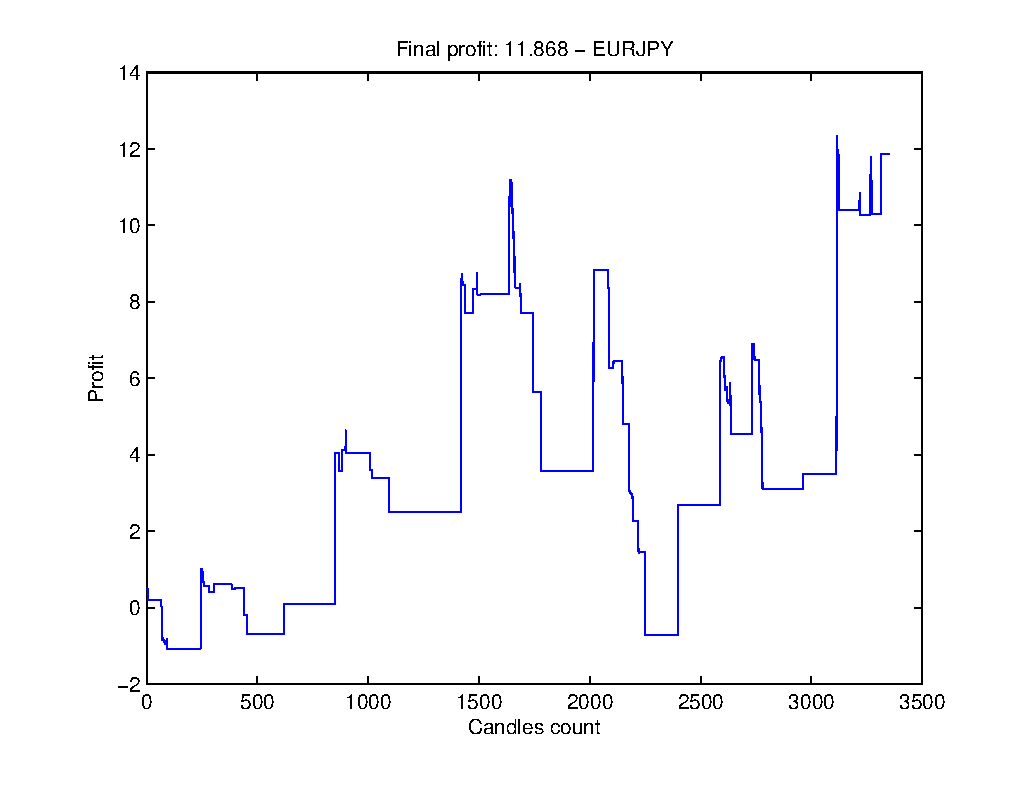
\includegraphics[width = 0.7\textwidth]{ROC_EURJPY_LS_SearchBestK_zysk.eps}
\caption{Cumulative return for the test period of EURJPY  while maximizing the profit}
\end{figure}
\FloatBarrier
\begin{verbatim}
LEARN PERIOD
The length of the cycle: 	89
Cumulative return: 	16.81
Calmar ratio: 	2.66
The number of opened long positions: 	100
The number of opened short positions:  	100

TEST PERIOD
The length of the cycle: 	89
Cumulative return: 	11.87
Calmar ratio: 	1.00
The number of opened long positions: 	61
The number of opened short positions: 	61
\end{verbatim}

\noindent \textbf{II The results of maximizing the Calmar ratio.}\\
\begin{figure}[h!]
\centering
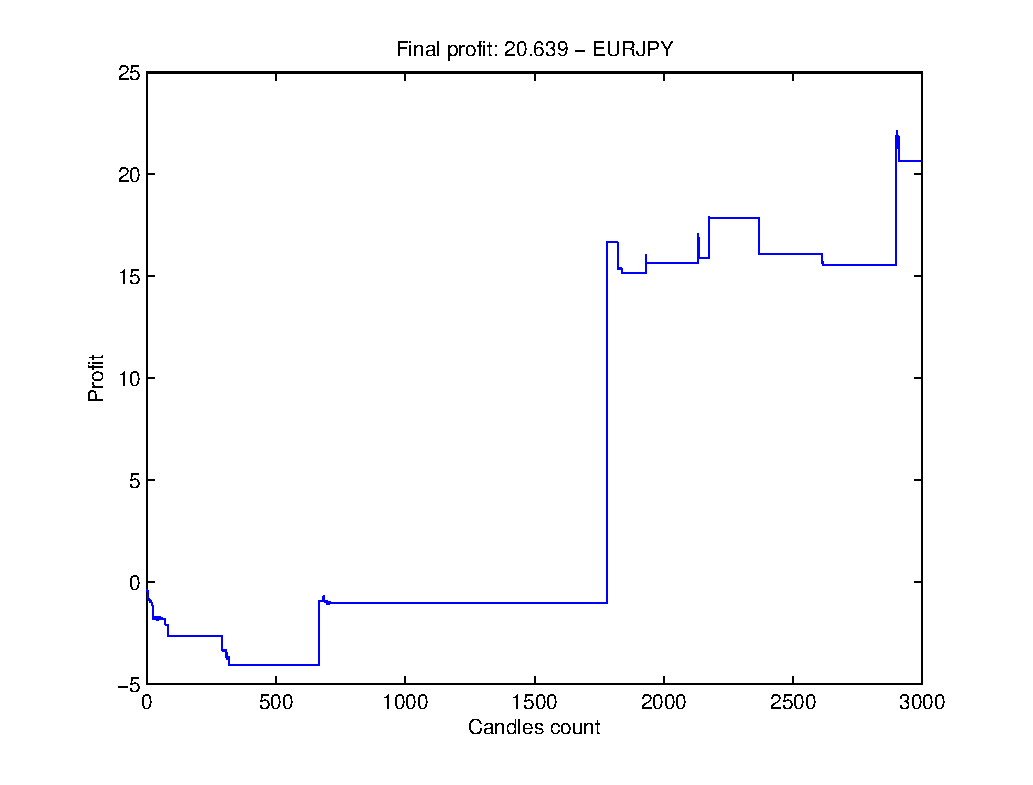
\includegraphics[width = 0.7\textwidth]{ROC_EURJPY_LS_SearchBestKCalmar_zysk.eps}
\caption{Cumulative return for the test period of EURJPY  while maximizing the Calmar ratio}
\end{figure}
\FloatBarrier
\begin{verbatim}
LEARN PERIOD
The length of the cycle: 	230
Cumulative return: 	12.82
Calmar ratio: 3.83
The number of opened long positions: 	52
The number of opened short positions:  	51

TEST PERIOD
The length of the cycle: 	230
Cumulative return: 	20.64
Calmar ratio: 	5.08
The number of opened long positions: 	28
The number of opened short positions: 	29
\end{verbatim}


\input{chapter1IndicatorsATR}
\section{OBV --- On Balance Volume}
\label{sec:1OBV}

On Balance Volume - równowaga wolumenu. Jest to wskaźnik opierający się na wolumenie. Sesjom wzrostowym towarzyszy wzrost wolumenu, natomiast sesjom zniżkowym spadek. Zmniejszanie obrotów przy wysokiem poziomie ceny instrumentu jest często interpretowane jako sygnał zmiany kierunku i zbliżających się sesjach spadkowych, a w przypadku spadków instrumentu i spadków obrotu, może to być sygnał, że jest to lokalny dołek i nastąpi zwrot ku górze. Istota wskaźnika polega na dodawaniu wolumenu przy sesjach wzrostowych wolumenu, a odejmowaniu wolumenu przy sesjach spadkowych.  OBV jest liczone według następujących reguł   : C  większa od ceny C [-1] to OBV = OBV [-1] + V, Jeżeli C mniejsza od C [-1] to OBV = OBV [-1] - V, Jeżeli C równa się C [-1] to OBV = OBV [-1]



\noindent

\noindent Poniższy listing przedstawia zaimplementowaną strategię w MATLAB-ie.
\begin{scriptsize}
\begin{lstlisting}

%Dane:
tStart=tic;

cSizes = size(C);
candlesCount = cSizes(1);
kon=candlesCount-1;

sumRa=zeros(1,candlesCount);
Ra=zeros(1,candlesCount);
pocz=50;
la=0; %liczba otwieranych pozycji
lastCandle = kon-16;
recordReturn=0; %rekord zysku
recordDrawdown=0; %rekord obsuniecia
pic1 = false;
obv=C(pocz-1,5)
for i=pocz:lastCandle
    
   
    
    
       if(C(i,4)>C(i-1,4))
       obv_tab(i)=obv+C(i,5);
       obv=obv_tab(i);
       end
       if(C(i,4)<C(i-1,4))
       obv_tab(i)=obv-C(i,5);
       obv=obv_tab(i);
       end
       
        
end

for i=100:lastCandle
obv_max(i)=max([obv_tab(i-14) obv_tab(i-13) obv_tab(i-12) obv_tab(i-11) obv_tab(i-10) obv_tab(i-9) obv_tab(i-8) obv_tab(i-7) obv_tab(i-6) obv_tab(i-5) obv_tab(i-4) obv_tab(i-3) obv_tab(i-2) obv_tab(i-1)]);
end



for i=100:lastCandle
    
    
            if (obv_tab(i)>obv_max(i))
            Ra(i)=C(i+1,4)-C(i+1,1)-spread; %zysk z i-tej pozycji long zamykanej na zamknieciu po paramADuration kroku
            
            la=la+1;
      
            end
    sumRa(i)=sumRa(i-1) + Ra(i); %krzywa narastania kapita3u
    
    if sumRa(i)>recordReturn
        recordReturn=sumRa(i);
    end
    
    if sumRa(i)-recordReturn<recordDrawdown
        recordDrawdown=sumRa(i)-recordReturn; %obsuniecie maksymalne
    end
end


\end{lstlisting}
\end{scriptsize}


Na podstawie zebranych informacji dotyczących wskaźnika $OBV$ utworzono prostą strategię inwestycyjną bazującą na regule: Obliczono maksymalną wartość OBV z 14 okresów i porównywano ją z wartością bieżącą OBV. Jeżeli wartość bieżąca OBV była większa od wartości maksymalnej z 14 okresów, to zawierano transakcję kupna. Badania zostały przeprowadzone na parze walutowej $EURCZK$ (szereg czasowy przedstawiony na rysunku \ref{rysunek2}). \\
\begin{figure}[h!]
\centering
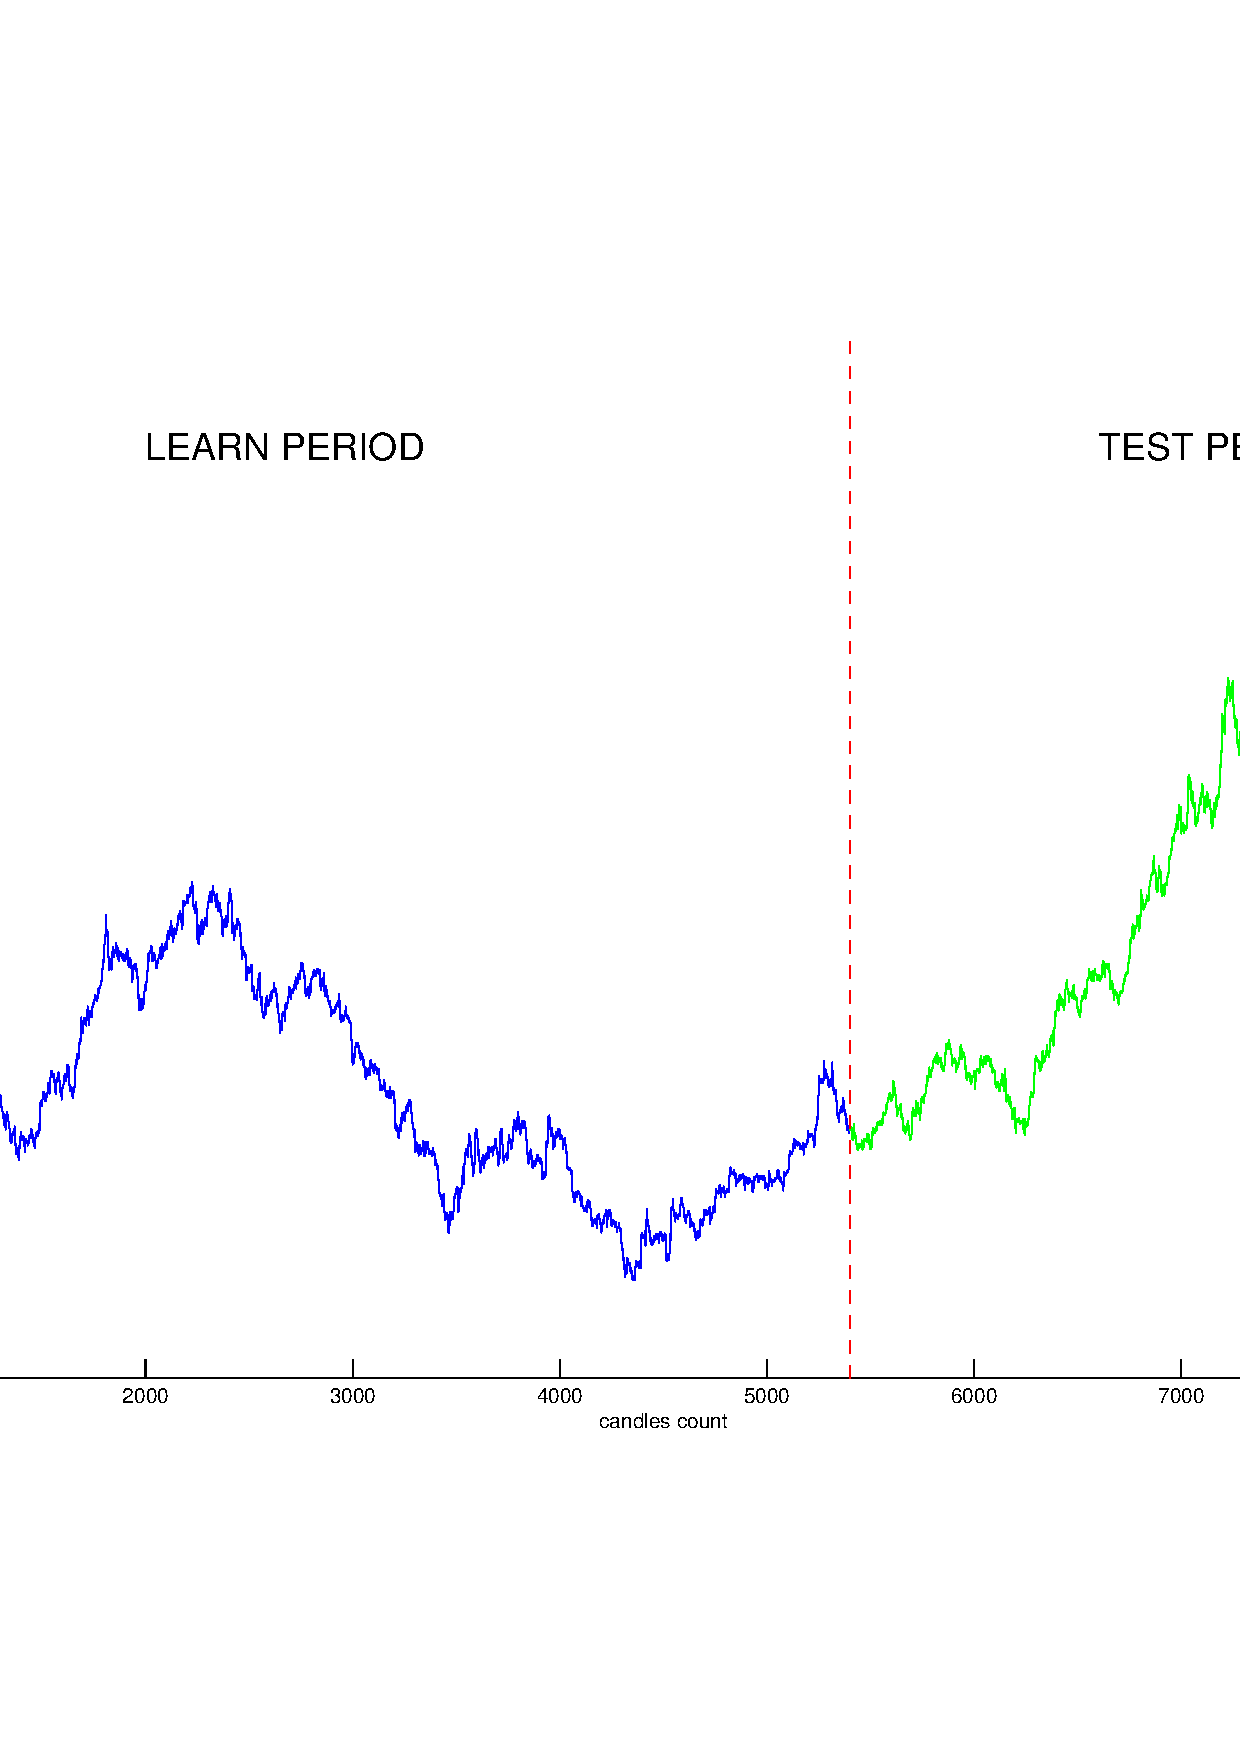
\includegraphics[width = \textwidth]{podzialDanych.png}
\caption{Badany szereg czasowy}
\label{rysunek2}
\end{figure}
\FloatBarrier
W przeprowadzonych badaniach przyjęto optymalną wartość parametru okresów do obliczenia wskaźnika OBV =14.
\newpage
\noindent \textbf{I Wyniki badań .}\\
\begin{figure}[h!]
\centering
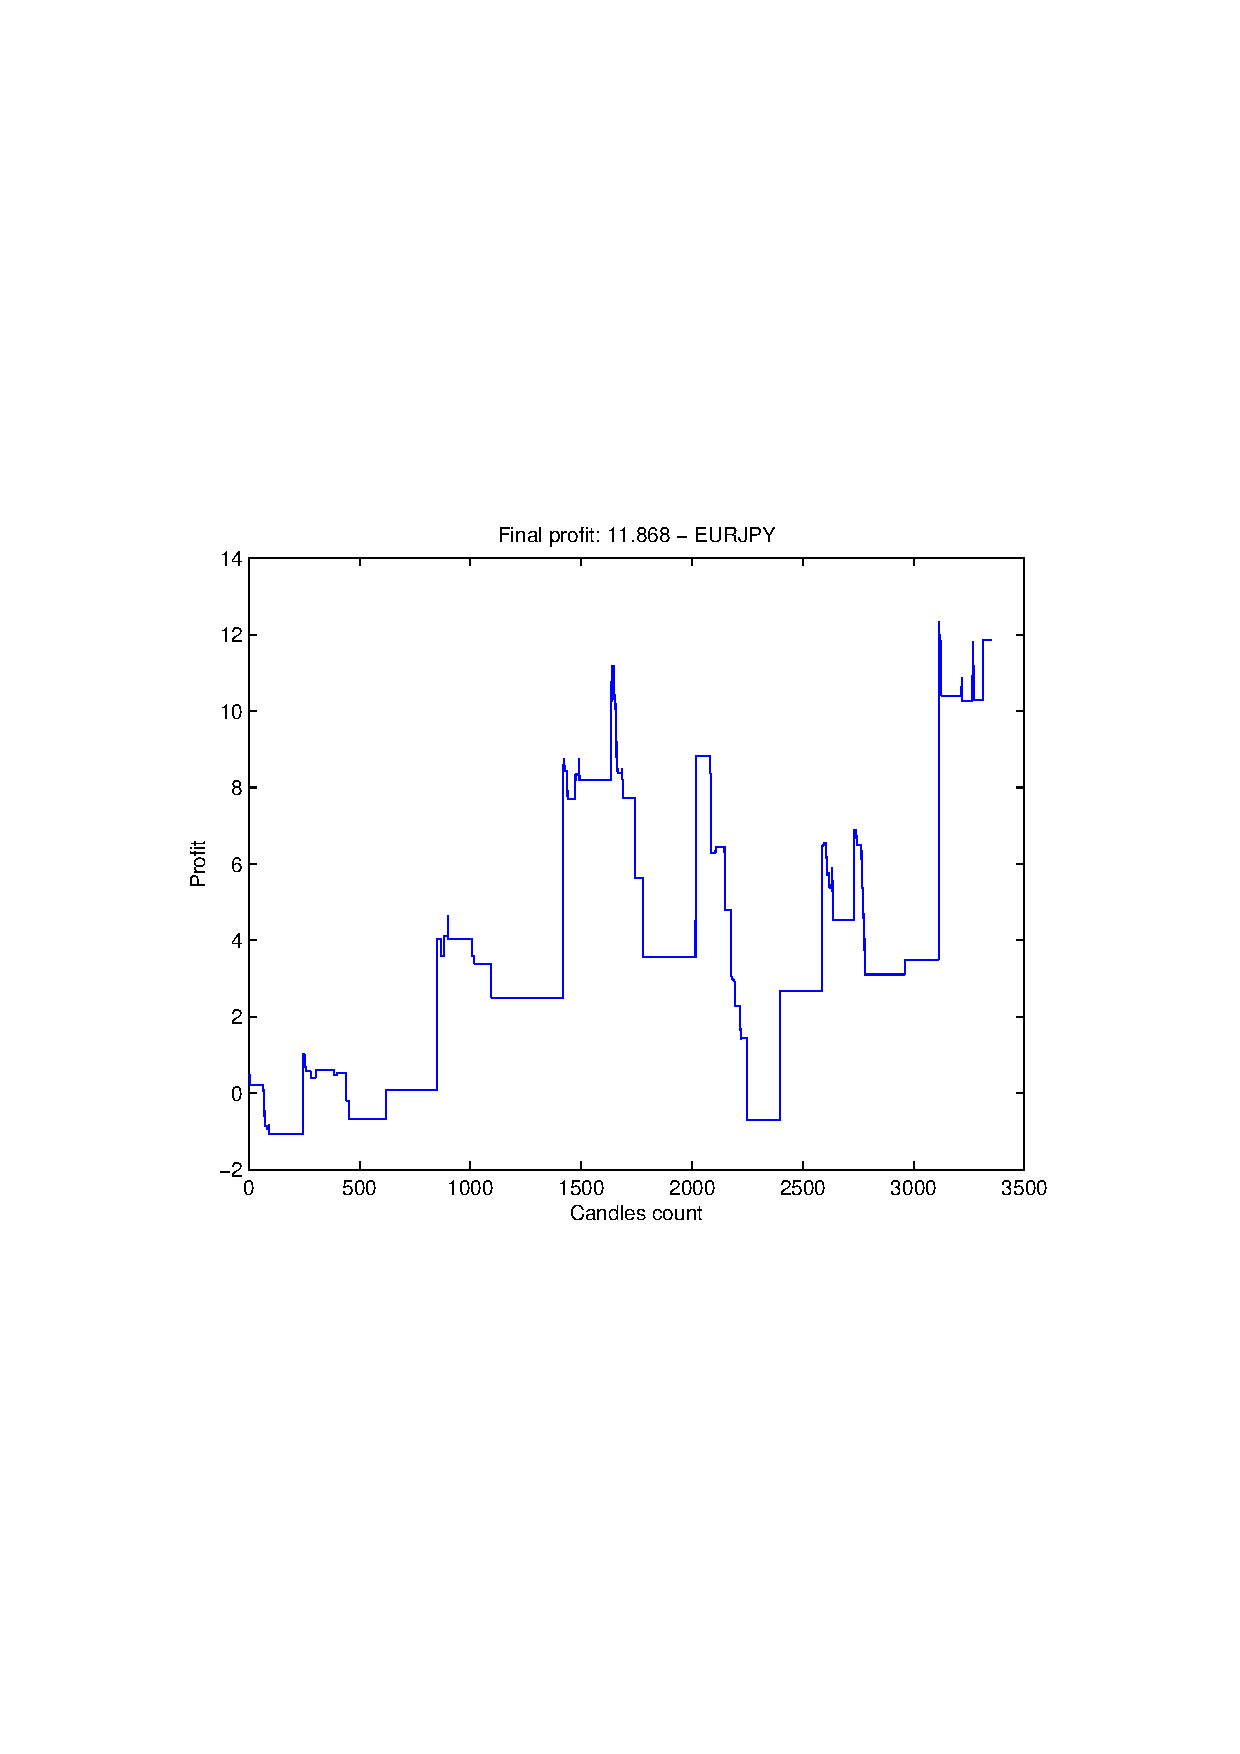
\includegraphics[width = 0.6\textwidth]{ROC_EURJPY_LS_SearchBestK_zysk.png}
\caption{Zysk skumulowany EURCZK na okresie testowym dla pozycji długich. }
\end{figure}
\FloatBarrier
\begin{verbatim}

Zysk skumulowany          7.1888
Calmar                    3.2053
liczba otwartych pozycji    1139





\end{verbatim}
%

\section{Stochastic Fast}
\label{sec:1STF}

Stochastic Fast - wskaźnik stochastyczny szybki, zaproponowany w latach 50-tych przez George C. Lane. Sposób wyliczenia wartości wskaźnika uwzględniając wartości O,H,C,L, polega na wyliczeniu dwóch linii. \ref{wzor_1} oraz \ref{wzor_2}.
\begin{equation}
ValK=100*[ \frac{C-Min(L;n)}{max(H;n - min(L;n)}]
\label{wzor_1}
\end{equation}
\begin{equation}
ValD=EMA(ValK;3)
\label{wzor_2}
\end{equation}
gdzie:
\begin{itemize}
\item ValD - jest wygładzoną linią ValK
\item n - ilość dni
\item EMA - Wykładnicza średnia krocząca(Exponential Moving Average)
\end{itemize}

\noindent Do podstawowych własności wskaźnika należą:
\begin{itemize}
\item opokazuje poziom dzisiejszego zamknięcia w stosunku do najniższego oraz najwyższego punktu w badanym okresie
\item porusza się w przedziale od 0-100
\item obliczamy 2 linie oscylatora ValK i ValD (Value K i Value D) uwzględniając, że ValK jest główną linią oscylatora natomiast ValD jest wygładzoną postacią ValK
\end{itemize}
Najważniejszą własnością opisywanego wskaźnika, stosowaną przy implementacjach strategii, jest fakt wskazywania momentów w których powinny zostać zawarte transakcje. 
\begin{itemize}
\item sygnałem kupna jest przecięcie linii ValK ponad ValD
\item sygnałem sprzedaży jest przecięcie linii ValK poniżej ValD.

\end{itemize}
\noindent Poniższy listing przedstawia zaimplementowaną strategię w środowisku MATLAB.
\begin{scriptsize}
\begin{lstlisting}
[a b]=size(C);
roz=(60*a)/100;
roz=round(roz);
paramSectionLearn = C(1:roz,:);

[m,n]=size(paramSectionLearn);

O=paramSectionLearn(:,1);
L=paramSectionLearn(:,3);
H=paramSectionLearn(:,2);
C=paramSectionLearn(:,4);

%Parametry 
spread=0.00016;
bestReturn = -100;
bestMa = 0;
%Część ucząca

countCandleLearn=m;
lastCandleLearn=0;
krok=1;
%Część valid

paramALengthT=0;
countCandleTest=m1;
lastCandleTest=0;
tmp=countCandleLearn-1;
ValK=zeros(1, countCandleLearn);
paramZakrespocz=0;
chwi=1;
for paramALengthL=40 %liczba świec wstecz ( do max)
        chwi=chwi;
        chwi
    paramZakrespocz(chwi)=paramALengthL;
   for i=2:tmp
       max3=max(H(max(i-paramALengthL, 1):i));
       min3=min(L(max(i-paramALengthL, 1):i));
      ValK(i)=100*(C(i)-min3)/(max3-min3);
   end
    ValD=ema(ValK,3);
    sumRa=zeros(1,tmp);
    Ra=zeros(1,tmp);
   lastCandleLearn=tmp;
       
%-------------obliczanie zysków
    WinReturn=0;
    DownReturn=0;
    CalmarLearn=0;
    BestCalLearn=0;
    
    for j=2:lastCandleLearn
        
        if ValK(j)>ValD(j) && ValK(j-1)<=ValD(j)
            Ra(j)=C(j+krok)-O(j+1)-spread ;% zysk z j-tej pozycji long zamykanej na zamknięciu po 1 kroku 
          else if ValK(j)<ValD(j) && ValK(j-1)>=ValD(j) 
            Ra(j)=-C(j+krok)+O(j+1)+spread; 
               end
        end
        sumRa(j)=sumRa(j-1)+Ra(j); %krzywa narastania kapitału
        
        if sumRa(j)>WinReturn
            WinReturn=sumRa(j);
        end
        
        DownReturnTmp=sumRa(j)-WinReturn;
        if  DownReturnTmp<DownReturn
            DownReturn= DownReturnTmp;
        end
     
    end
    chwi=chwi+1;   
sumFinal=sumRa(lastCandleLearn);
CalmarLearn=-sumFinal/DownReturn;

if bestReturn < sumFinal
    bestMa=paramALengthL;
end
end

sumFinal=sumRa(lastCandleLearn);
CalmarLearn=-sumFinal/DownReturn;
\end{lstlisting}
\end{scriptsize}

Na podstawie zebranych informacji dotyczących wskaźnika Stochastic Fast, stworzono powyższy program uwzględniając pozycje sprzedaży i kupna przy określonych przecięciach. Badania przeprowadzono na rynku usdjpy.
\begin{itemize}
\item sygnałem kupna jest przecięcie linii ValK ponad ValD
\item sygnałem sprzedaży jest przecięcie linii ValK poniżej ValD.
\end{itemize}
Podczas badania wskaźnika cały zbiór danych (świec) podzielony został na dwie części: uczącą ($60\%$ całości) oraz testową ($40\%$ całości). W przeprowadzonych badaniach poszukiwano optymalnej wartości parametru $k$ na okresie uczącym, następnie weryfikowano otrzymane wyniki na okresie testowym. Wybór optymalnej wartości parametru (dla czystego wskaźnika Ma) polegał na wyszukaniu najlepszego zysku. \\
\newpage
\noindent \textbf{\\Wyniki badań przy maksymalizacji po zysku.}\\
\begin{figure}[h!]
\centering
\includegraphics[scale=0.6]{SF_zysk_us.png}\\
\caption{Zysk}
\end{figure}
\FloatBarrier
\noindent \textbf{Wycinek ValK i ValD}\\
\begin{figure}[h!]
\centering
\includegraphics[scale=0.4]{ValD_ValK_us.png}
\caption{ValD - kolor niebieski, ValK - kolor czerowny }
\end{figure}
\FloatBarrier
%

\input{chapter1IndicatorsPPV}
\section{MACD --- Moving Average Covergence Divergence}
\label{sec:1MACD}

Average True Range - średni zakres zmian. Jest to wskaźnik obliczający zmienność cen w ujęciu bezwględnym.  Wykorzystywany jest do wychwycenia zmienności kursu. Wskaźnik ATR oblicza się jako średnią z rzeczywistego zakresu zmian (TR - True Range), który jest największą wartością z następujących trzech wielkości : odległością pomiędzy poprzednią ceną zamknięcia (Close) a dzisiejszym minimum (Low),odległością pomiędzy dzisiejszym maksimum (High) a poprzednią ceną zamknięcia (Close),odległością pomiędzy dzisiejszym maksimum (High) i minimum (Low). Wskaźnik jest używany do przewidywania lokalnych szczytów i dołków - jego wartość jest często wysoka i osiąga szczyt przed lokalnym minimum lub maksimum kursu . Także wysoka wartość wskaźnika podczas gwałtownego spadku lub wzrostu może zapowiadać dłuższą zmianę trendu. Niskie wartości wskaźnika potwierdzają trend horyzontalny.



\noindent

\noindent Poniższy listing przedstawia zaimplementowaną strategię w MATLAB-ie.
\begin{scriptsize}
\begin{lstlisting}


%Dane:
tStart=tic;
cSizes = size(C);
candlesCount = cSizes(1);
kon=candlesCount-1;
sumRa=zeros(1,candlesCount);
Ra=zeros(1,candlesCount);
pocz=50;
la=0; %liczba otwieranych pozycji
lastCandle = kon-16;
recordReturn=0; %rekord zysku
recordDrawdown=0; %rekord obsuniecia
pic1 = false;
obv=C(pocz-1,5)
for i=pocz:lastCandle
 
   
    
    
       if(C(i,4)>C(i-1,4))
       obv_tab(i)=obv+C(i,5);
       obv=obv_tab(i);
       end
       if(C(i,4)<C(i-1,4))
       obv_tab(i)=obv-C(i,5);
       obv=obv_tab(i);
       end
       
        
end

for i=100:lastCandle
obv_max(i)=max([obv_tab(i-14) obv_tab(i-13) obv_tab(i-12) obv_tab(i-11) obv_tab(i-10) obv_tab(i-9) obv_tab(i-8) obv_tab(i-7) obv_tab(i-6) obv_tab(i-5) obv_tab(i-4) obv_tab(i-3) obv_tab(i-2) obv_tab(i-1)]);
end

for i=100:lastCandle
    
    
            if (obv_tab(i)>obv_max(i))
            Ra(i)=C(i+1,4)-C(i+1,1)-spread; %zysk z i-tej pozycji long zamykanej na zamknieciu po paramADuration kroku
            
            la=la+1;
      
            end
    sumRa(i)=sumRa(i-1) + Ra(i); %krzywa narastania kapita3u
    
    if sumRa(i)>recordReturn
        recordReturn=sumRa(i);
    end
    
    if sumRa(i)-recordReturn<recordDrawdown
        recordDrawdown=sumRa(i)-recordReturn; %obsuniecie maksymalne
    end
end

sumReturn=sumRa(lastCandle);




\end{lstlisting}
\end{scriptsize}


Na podstawie zebranych informacji dotyczących wskaźnika $ATR$ utworzono prostą strategię inwestycyjną bazującą na regule: Obliczono średnią ATR z 14 okresów i porównywano ją z wartością bezwględną z różnicy pomiędzy ceną otwarcia z aktualnej świecy, a ceną zaknięcia z poprzedzającej ceny. Jeżeli średnia była większa od wartości bezwględnej to zawierano transakcję kupna. Badania zostały przeprowadzone na parze walutowej $EURCZK$ (szereg czasowy przedstawiony na rysunku \ref{rysunek2}). \\
\begin{figure}[h!]
\centering
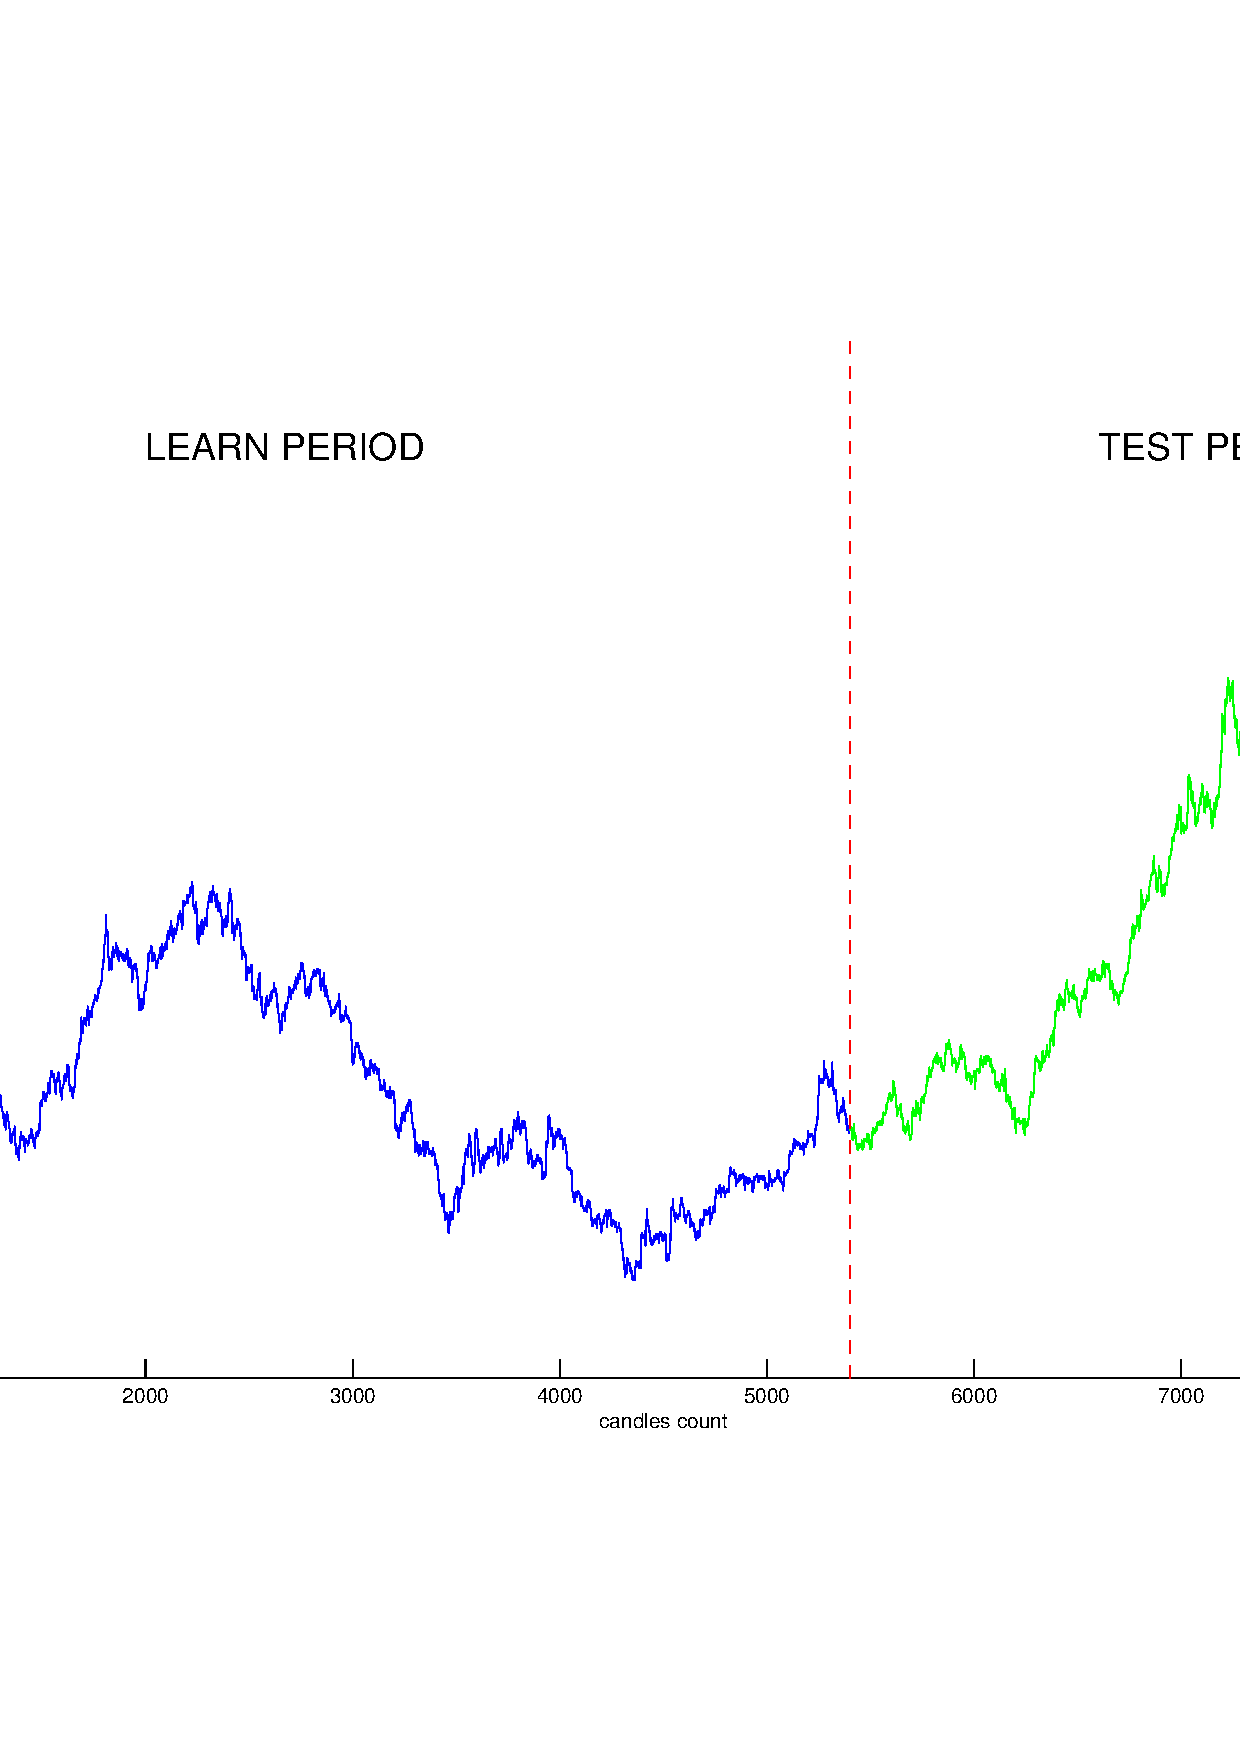
\includegraphics[width = \textwidth]{podzialDanych.png}
\caption{Badany szereg czasowy}
\label{rysunek2}
\end{figure}
\FloatBarrier
W przeprowadzonych badaniach przyjęto optymalną wartość parametru okresów do obliczenia wskaźnika ATR =14, następnie weryfikowano otrzymane wyniki na okresie testowym. 
\newpage
\noindent \textbf{I Wyniki badań .}\\
\begin{figure}[h!]
\centering
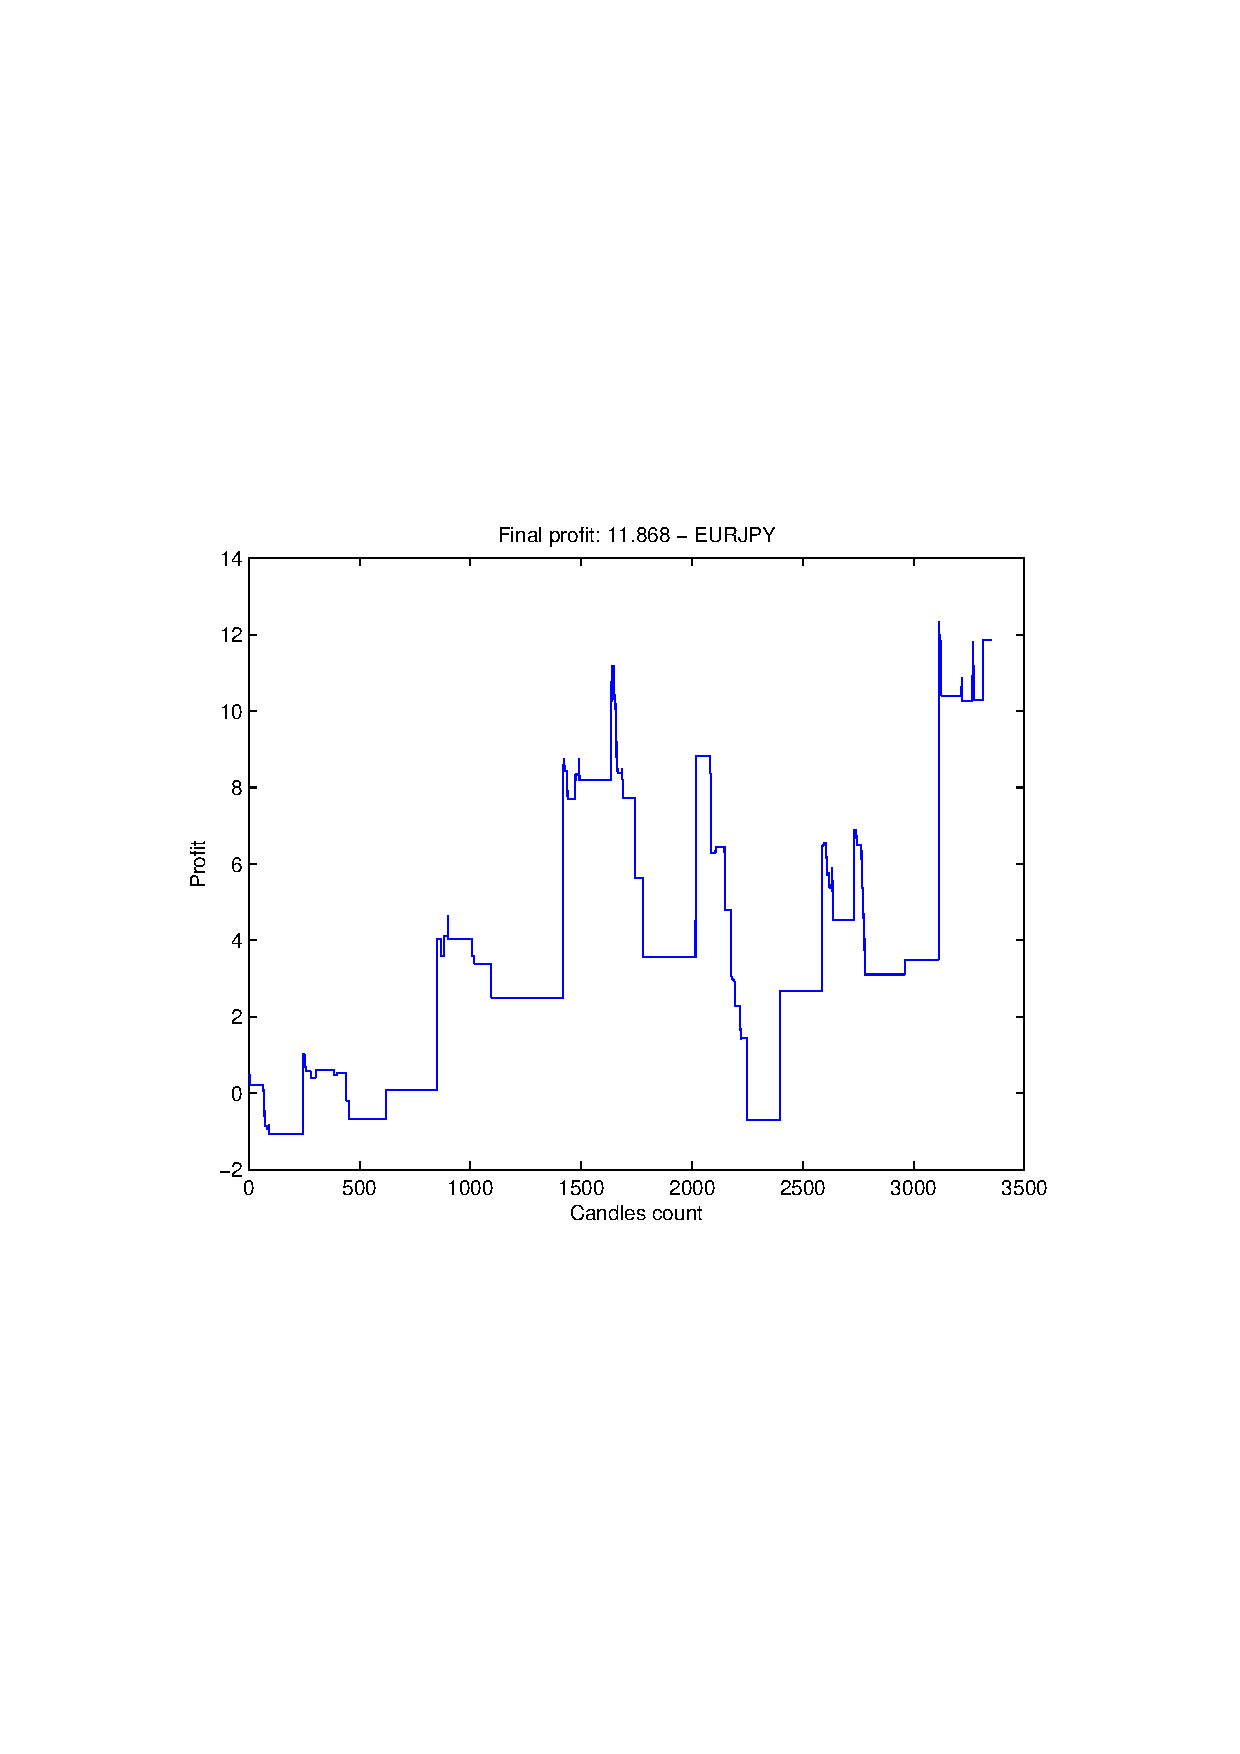
\includegraphics[width = 0.6\textwidth]{ROC_EURJPY_LS_SearchBestK_zysk.png}
\caption{Zysk skumulowany EURCZK na okresie testowym dla pozycji długich. }
\end{figure}
\FloatBarrier
\begin{verbatim}

Zysk skumulowany          18.4184
Calmar                     2.3641
liczba otwartych pozycji  8777




\end{verbatim}
%

\section{Stochastic Slow}
\label{sec:1STS}

Stochastic Slow jest wolniejszą wersja podstawowego oscylatora stochastycznego. Składa się z dwóch linii oscylacyjnych: głównej linii oscylatora tzw. \%K oraz pomocniczej wygładzonej postaci tej linii tzw. \%D. Obie linie osiągają wartości z przedziału 0 - 100.  Sposób wyliczenia kolejnych wartości obu linii dla danego punktu w czasie przedstawiają wzory \ref{wzor_1} oraz \ref{wzor_2}.
\begin{equation}
\%K = \left[\begin{array}{c} \frac{ \sum_{j=0}^{2} (C_j - min(L_j, n))}{ \sum_{j=0}^{2} (max(H_j, n) - min(L_j, n))}\end{array}\right]\\
\label{wzor_1}
\end{equation}
\begin{equation}
\%D = SMA(\%K, 3)
\label{wzor_2}
\end{equation}

\noindent Dodatkowo mogą być poszukiwane dywergencje względem wykresu cenowego. Możliwe jest też poszukiwanie tzw. odwróconych dywergencji. W tej wersji wskaźnik może być używany jako miernik wykupienia / wyprzedania rynku. Wadą wskaźnika jest to, że w mocnych ruchach trendowych skrajne stany rynku mogą być sygnalizowane przedwcześnie.
Przy interpretacji wskaźnika najważniejszy jednak jest fakt, że wskazuje on momenty w których mogą być zawierane transakcje. Podstawowa zasada zakłada przyjęcie jako sygnału kupna sytuację gdy występują przecięcia linii \%D przez linię \%K od dołu. Natomiast, gdy linia \%D jest przecinana przez linię \%K od góry, to przyjmuje się taką sytuację za sygnał sprzedaży. Zostało to przedstawione na rysunku \ref{zasada}. \\
\begin{figure}[h!]
\centering
\includegraphics[width = \textwidth]{ss.png}
\caption{Fragment przebiegu kursu akcji (górny wykres) oraz odpowiadające jemu linie \%K i \%D wraz z sygnałami kupna --- błękitne strzałki oraz sygnałami sprzedaży --- pomarańczowe strzałki (dolny wykres)}
\label{zasada}
\end{figure}
\FloatBarrier

\noindent Poniższy listing przedstawia zaimplementowaną w środowisku MATLAB strategię wykorzystującą opisywany wskaźnik.
\begin{scriptsize}
\begin{lstlisting}
maxes=zeros(candlesCount,1);
mins=zeros(candlesCount,1);
K=zeros(candlesCount,1);
D=zeros(candlesCount,1);
kon=candlesCount-1;
for i=4:kon
    maxes(i) = max(verificationC(i-min(i-1,paramMALength):i-1,2));
    mins(i) = min(verificationC(i-min(i-1,paramMALength):i-1,3));
    K(i) = 100 * (sum(verificationC(i-min(i-1,3):i-1,4)-mins(i-min(i-1,2):i)) / sum(maxes(i-min(i-1,2):i)-mins(i-min(i-1,2):i)));
    D(i) = sum(K(i-min(i-1,2):i)) / min(i-1,3);
end

sumR=zeros(1,candlesCount);
R=zeros(1,candlesCount);
pocz=max(paramMALength, 10)+3;
iL=0; %liczba otwieranych pozycji kupna
iS=0; %liczba otwieranych pozycji sprzedarzy
lastCandle = kon-paramMALength;
recordReturn=0;  %rekord zysku
recordDrawdown=0;  %rekord obsuniecia
LastPos = 0; % zmienna do prz echowywa nia warto ś ci na otwarciu ostatniej pozycji
for i=pocz:lastCandle
    
    if K(i-1) < D(i-1) && K(i) >= D(i) % warunek kupna
        R(i)= - C(i+1,4)+LastPos-spread; % zamknięcie S
        LastPos = C(i+1,1); % otwarcie L
        iL=iL+1;
    elseif K(i-1) > D(i-1) && K(i) <= D(i) % warunek sprzedaż y
        R(i)=C(i+1,4)-LastPos-spread; % zamknięcie L
        LastPos = C(i+1,1); % otwarcie S
        iS=iS+1;
    end
    sumR(i)= sum(R(pocz:i));  %krzywa narastania kapitału
    
    if sumR(i)>recordReturn
        recordReturn=sumR(i);
    end
    
    if sumR(i)-recordReturn<recordDrawdown
        recordDrawdown=sumR(i)-recordReturn;  %obsuniecie maksymalne
    end
end

%wyniki końcowe
sumReturn=sumR(lastCandle);
Calmar=-sumReturn/recordDrawdown;  %wskaznik Calmara
\end{lstlisting}
\end{scriptsize}


Na podstawie zebranych informacji dotyczących wskaźnika $Stochastic Slow$ utworzono prostą strategię inwestycyjną bazującą na regule: jeśli linia $\%D$ jest przecinana przez  linię $\%K$ od dołu, to otwierana jest pozycja długa ($L$), a zamykana pozycja krótka ($S$), która została wcześniej otwarta. Natomiast gdy linia \%D jest przecinana przez linię \%K od góry, to otwarta zostanie pozycja krótka, a zamknięta długa. Badania zostały przeprowadzone na parze walutowej $CADCHF$ (szereg czasowy przedstawiony na rysunku \ref{rys2}). \\
\begin{figure}[h!]
\centering
\includegraphics[width = \textwidth]{szereg.png}
\caption{Badany szereg czasowy z podziałem na część uczącą i testową}
\label{rys2}
\end{figure}
\FloatBarrier
Cały zbiór danych (świec) podzielony został na dwie części: uczącą ($60\%$ całości) oraz testową ($40\%$ całości). W przeprowadzonych badaniach poszukiwano optymalnej wartości parametru $n$ na okresie uczącym, następnie weryfikowano otrzymane wyniki na okresie testowym. Wybór optymalnej wartości parametru $n$ determinowano na dwa sposoby:
\begin{itemize}
\item otrzymanego zysku skumulowanego,
\item wskaźnika Calamara.
\end{itemize}

\noindent \textbf{I Wyniki badań przy maksymalizacji po zysku.}\\
\begin{figure}[h!]
\centering
\includegraphics[width = 0.6\textwidth]{SS_CADCHF_S4LS_zysk.png}
\caption{Zysk skumulowany CADCHF na okresie testowym przy maksymalizacji według zysku}
\end{figure}
\FloatBarrier
\begin{verbatim}
OKRES UCZĄCY
Zysk skumulowany:     0.2917
Calmar:     0.4538
Liczba otwartych pozycji długich:     400
Liczba otwartych pozycji krótkich:     405

OKRES WALIDUJĄCY
Zysk skumulowany:     -1.3244
Calmar:     -1
Liczba otwartych pozycji długich:     244
Liczba otwartych pozycji krótkich:     245
\end{verbatim}
\newpage
\textbf{II Wyniki badań przy maksymalizacji po wskaźniku Calmara.}\\
\begin{figure}[h!]
\centering
\includegraphics[width = 0.6\textwidth]{SS_CADCHF_S4LS_calmar.png}
\caption{Zysk skumulowany EURJPY na okresie testowym przy maksymalizacji według Calmara}
\end{figure}
\FloatBarrier
\begin{verbatim}
OKRES UCZĄCY
Zysk skumulowany:     0.2917
Calmar:     0.4538
Liczba otwartych pozycji długich:     400
Liczba otwartych pozycji krótkich:     405

OKRES WALIDUJĄCY
Zysk skumulowany:     -1.3244
Calmar:     -1
Liczba otwartych pozycji długich:     244
Liczba otwartych pozycji krótkich:     245
\end{verbatim}
%

\section{Mass Index}
\label{sec:1ATR}

Mass Index wskaźnik jest pomocny w identyfikacji punktów zwrotnych, poprzez mierzenie odległości pomiędzy cenami maksymalnymi a minimalnymi. Według autora zmiana kierunku trendu następuje w momencie zaobserwowania tzw. wybrzuszenia zwrotnego, czyli wejścia wskaźnika ponad poziom 27 i następnie spadku poniżej 26,5. Wskaźnik nie identyfikuje jednak kierunku trendu, ustala jedynie punkt zwrotny. Sposób wyliczenia kolejnych wartości wskaźnika dla danego punktu w czasie przedstawia wzór \ref{wzor_3}.
\begin{equation}
Mass Index = \sum_{0}^{24} \left[\begin{array}{c} \frac{ EMA(H - L, 9)}{ EMA(EMA(H-L, 9), 9)}\end{array}\right]\\
\label{wzor_3}
\end{equation}

\noindent Sama interpretacja wskaźnika nie pozwala na wskazanie momentów w których mogą być zawierane konkretne transakcje (kopno/sprzedarz). W określeniu czy jest to sygnał kupna czy sprzedaży autor zaleca stosowanie 9- dniowej ekspotencjalnej średniej na wykresie notowań. Dlatego przyjeliśmy zasadę, która zakłada, że po wystąpieniu wybrzuszenia zwrotnego przyjmujemy jako sygnał kupna sytuację gdy wartość ceny zamknięcia przewyższa wartość 9- dniowej ekspotencjalnej średniej. Natomiast, gdy wartość ceny zamknięcia jest mniejsza od wartość 9- dniowej ekspotencjalnej średniej, to przyjmuje się taką sytuację za sygnał sprzedaży. Zostało to przedstawione na rysunku \ref{kupsprz2}. \\
\begin{figure}[h!]
\centering
\includegraphics[width = \textwidth]{mi2.png}
\caption{Fragment przebiegu kursu akcji z naniesioną  9- dniową ekspotencjalną średnią (górny wykres) oraz odpowiadające jemu wartości wskaźnika indeksu masy wraz z sygnałami kupna --- zielone strzałki oraz sygnałami sprzedaży --- czerwone strzałki (dolny wykres)}
\label{kupsprz2}
\end{figure}
\FloatBarrier

\noindent Poniższy listing przedstawia zaimplementowaną w środowisku MATLAB strategię wykorzystującą opisywany wskaźnik.
\begin{scriptsize}
\begin{lstlisting}
bestiL = 0;
bestiS = 0;
HL = C(:,2) - C(:,3); % różnica H - L
kon=candlesCount-1;
MI = zeros(candlesCount,1);
HLaverage = ema(HL,9);
EMA2 = HLaverage(9:end) ./ ema(HLaverage(9:end),9);
for i = 41:kon-16
    MI(i) = sum(EMA2(i-24:i));
end
Caverages = ema(C(:,4),9);

sumR=zeros(1,candlesCount);
R=zeros(1,candlesCount);
pocz=50;
iL=0; %liczba otwieranych pozycji kupna
iS=0; %liczba otwieranych pozycji sprzedarzy
lastCandle = kon-16;
recordReturn=0;  %rekord zysku
recordDrawdown=0;  %rekord obsuniecia
LastPos = 0;
pic1 = false;

for i=pocz:lastCandle
    
    if pic1 == false && MI(i) > 27 % warunek wystąpienia wybrzuszenia zwrotnego
        pic1 = true;
    end
    if pic1 == true && MI(i) < 26.5 % warunek zawarcia transakcji
        if C(i,4) > Caverages(i) % warunek kupna
            R(i)= -C(i+1,4)-LastPos-spread; % zamknięcie S
            LastPos = C(i+1,1); % otwarcie L
            iL=iL+1;
        elseif C(i,4) < Caverages(i) % warunek sprzedaży
            R(i)=C(i+1,4)-LastPos-spread; % zamknięcie L
            LastPos = C(i+1,1); % otwarcie S
            iS=iS+1;
        end
        pic1 = false;
    end
    sumR(i)= sum(R(pocz:i));  %krzywa narastania kapitału
    
    if sumR(i)>recordReturn
        recordReturn=sumR(i);
    end
    
    if sumR(i)-recordReturn<recordDrawdown
        recordDrawdown=sumR(i)-recordReturn;  %obsuniecie maksymalne
    end
end

%wyniki końcowe
sumReturn=sumR(lastCandle);
Calmar=-sumReturn/recordDrawdown;  %wskaznik Calmara
\end{lstlisting}
\end{scriptsize}


Na podstawie zebranych informacji dotyczących wskaźnika $Mass Index$ utworzono prostą strategię inwestycyjną bazującą na regule: jeśli wystąpi wybrzuszenie zwrotne oraz wartość ceny zamknięcia przewyższy wartość 9- dniowej ekspotencjalnej średniej, to otwierana jest pozycja długa ($L$), a zamknięta pozycja krótka ($S$), która została wcześniej otwarta . Natomiast, gdy wartość ceny zamknięcia będzie mniejsza od wartość 9- dniowej ekspotencjalnej średniej, to otwarta zostanie pozycja krótka ($S$), a zamknięta długa. Badania zostały przeprowadzone na parze walutowej $CADCHF$ (szereg czasowy przedstawiony na rysunku \ref{rys2}). \\

Ze względu na to iż wszystkie parametry wzoru są arbitralnie ustawione, to zbiór danych (świec) nie został podzielony na dwie części: uczącą i testującą ($40\%$ całości). Na całym zbiorze danych weryfikowano skuteczność strategii. \\


\newpage
\noindent \textbf{I Wyniki badań.}\\
\begin{figure}[h!]
\centering
\includegraphics[width = 0.6\textwidth]{MI_CADCHF_S4LS.png}
\caption{Zysk skumulowany CADCHF na okresie testowym przy maksymalizacji według zysku}
\end{figure}
\FloatBarrier
\begin{verbatim}
OKRES WALIDUJĄCY
Zysk skumulowany:     -8.3942
Calmar:     -1
Liczba otwartych pozycji długich:     5
Liczba otwartych pozycji krótkich:     3
\end{verbatim}
%


\include{chapter3SimpleRules}
%\appendix
%\include{appendix}

\backmatter%%%%%%%%%%%%%%%%%%%%%%%%%%%%%%%%%%%%%%%%%%%%%%%%%%%%%%%
\include{solutions}
\include{referenc}
\printindex

%%%%%%%%%%%%%%%%%%%%%%%%%%%%%%%%%%%%%%%%%%%%%%%%%%%%%%%%%%%%%%%%%%%%%%

\end{document}





